\documentclass[]{article}
\usepackage{lmodern}
\usepackage{amssymb,amsmath}
\usepackage{ifxetex,ifluatex}
\usepackage{fixltx2e} % provides \textsubscript
\ifnum 0\ifxetex 1\fi\ifluatex 1\fi=0 % if pdftex
  \usepackage[T1]{fontenc}
  \usepackage[utf8]{inputenc}
\else % if luatex or xelatex
  \ifxetex
    \usepackage{mathspec}
  \else
    \usepackage{fontspec}
  \fi
  \defaultfontfeatures{Ligatures=TeX,Scale=MatchLowercase}
\fi
% use upquote if available, for straight quotes in verbatim environments
\IfFileExists{upquote.sty}{\usepackage{upquote}}{}
% use microtype if available
\IfFileExists{microtype.sty}{%
\usepackage{microtype}
\UseMicrotypeSet[protrusion]{basicmath} % disable protrusion for tt fonts
}{}
\usepackage[margin=1in]{geometry}
\usepackage{hyperref}
\hypersetup{unicode=true,
            pdftitle={Assignment 1: Printed circuits},
            pdfauthor={Pranav Kasela - 846965},
            pdfborder={0 0 0},
            breaklinks=true}
\urlstyle{same}  % don't use monospace font for urls
\usepackage{color}
\usepackage{fancyvrb}
\newcommand{\VerbBar}{|}
\newcommand{\VERB}{\Verb[commandchars=\\\{\}]}
\DefineVerbatimEnvironment{Highlighting}{Verbatim}{commandchars=\\\{\}}
% Add ',fontsize=\small' for more characters per line
\usepackage{framed}
\definecolor{shadecolor}{RGB}{248,248,248}
\newenvironment{Shaded}{\begin{snugshade}}{\end{snugshade}}
\newcommand{\KeywordTok}[1]{\textcolor[rgb]{0.13,0.29,0.53}{\textbf{#1}}}
\newcommand{\DataTypeTok}[1]{\textcolor[rgb]{0.13,0.29,0.53}{#1}}
\newcommand{\DecValTok}[1]{\textcolor[rgb]{0.00,0.00,0.81}{#1}}
\newcommand{\BaseNTok}[1]{\textcolor[rgb]{0.00,0.00,0.81}{#1}}
\newcommand{\FloatTok}[1]{\textcolor[rgb]{0.00,0.00,0.81}{#1}}
\newcommand{\ConstantTok}[1]{\textcolor[rgb]{0.00,0.00,0.00}{#1}}
\newcommand{\CharTok}[1]{\textcolor[rgb]{0.31,0.60,0.02}{#1}}
\newcommand{\SpecialCharTok}[1]{\textcolor[rgb]{0.00,0.00,0.00}{#1}}
\newcommand{\StringTok}[1]{\textcolor[rgb]{0.31,0.60,0.02}{#1}}
\newcommand{\VerbatimStringTok}[1]{\textcolor[rgb]{0.31,0.60,0.02}{#1}}
\newcommand{\SpecialStringTok}[1]{\textcolor[rgb]{0.31,0.60,0.02}{#1}}
\newcommand{\ImportTok}[1]{#1}
\newcommand{\CommentTok}[1]{\textcolor[rgb]{0.56,0.35,0.01}{\textit{#1}}}
\newcommand{\DocumentationTok}[1]{\textcolor[rgb]{0.56,0.35,0.01}{\textbf{\textit{#1}}}}
\newcommand{\AnnotationTok}[1]{\textcolor[rgb]{0.56,0.35,0.01}{\textbf{\textit{#1}}}}
\newcommand{\CommentVarTok}[1]{\textcolor[rgb]{0.56,0.35,0.01}{\textbf{\textit{#1}}}}
\newcommand{\OtherTok}[1]{\textcolor[rgb]{0.56,0.35,0.01}{#1}}
\newcommand{\FunctionTok}[1]{\textcolor[rgb]{0.00,0.00,0.00}{#1}}
\newcommand{\VariableTok}[1]{\textcolor[rgb]{0.00,0.00,0.00}{#1}}
\newcommand{\ControlFlowTok}[1]{\textcolor[rgb]{0.13,0.29,0.53}{\textbf{#1}}}
\newcommand{\OperatorTok}[1]{\textcolor[rgb]{0.81,0.36,0.00}{\textbf{#1}}}
\newcommand{\BuiltInTok}[1]{#1}
\newcommand{\ExtensionTok}[1]{#1}
\newcommand{\PreprocessorTok}[1]{\textcolor[rgb]{0.56,0.35,0.01}{\textit{#1}}}
\newcommand{\AttributeTok}[1]{\textcolor[rgb]{0.77,0.63,0.00}{#1}}
\newcommand{\RegionMarkerTok}[1]{#1}
\newcommand{\InformationTok}[1]{\textcolor[rgb]{0.56,0.35,0.01}{\textbf{\textit{#1}}}}
\newcommand{\WarningTok}[1]{\textcolor[rgb]{0.56,0.35,0.01}{\textbf{\textit{#1}}}}
\newcommand{\AlertTok}[1]{\textcolor[rgb]{0.94,0.16,0.16}{#1}}
\newcommand{\ErrorTok}[1]{\textcolor[rgb]{0.64,0.00,0.00}{\textbf{#1}}}
\newcommand{\NormalTok}[1]{#1}
\usepackage{graphicx,grffile}
\makeatletter
\def\maxwidth{\ifdim\Gin@nat@width>\linewidth\linewidth\else\Gin@nat@width\fi}
\def\maxheight{\ifdim\Gin@nat@height>\textheight\textheight\else\Gin@nat@height\fi}
\makeatother
% Scale images if necessary, so that they will not overflow the page
% margins by default, and it is still possible to overwrite the defaults
% using explicit options in \includegraphics[width, height, ...]{}
\setkeys{Gin}{width=\maxwidth,height=\maxheight,keepaspectratio}
\IfFileExists{parskip.sty}{%
\usepackage{parskip}
}{% else
\setlength{\parindent}{0pt}
\setlength{\parskip}{6pt plus 2pt minus 1pt}
}
\setlength{\emergencystretch}{3em}  % prevent overfull lines
\providecommand{\tightlist}{%
  \setlength{\itemsep}{0pt}\setlength{\parskip}{0pt}}
\setcounter{secnumdepth}{0}
% Redefines (sub)paragraphs to behave more like sections
\ifx\paragraph\undefined\else
\let\oldparagraph\paragraph
\renewcommand{\paragraph}[1]{\oldparagraph{#1}\mbox{}}
\fi
\ifx\subparagraph\undefined\else
\let\oldsubparagraph\subparagraph
\renewcommand{\subparagraph}[1]{\oldsubparagraph{#1}\mbox{}}
\fi

%%% Use protect on footnotes to avoid problems with footnotes in titles
\let\rmarkdownfootnote\footnote%
\def\footnote{\protect\rmarkdownfootnote}

%%% Change title format to be more compact
\usepackage{titling}

% Create subtitle command for use in maketitle
\newcommand{\subtitle}[1]{
  \posttitle{
    \begin{center}\large#1\end{center}
    }
}

\setlength{\droptitle}{-2em}

  \title{Assignment 1: Printed circuits}
    \pretitle{\vspace{\droptitle}\centering\huge}
  \posttitle{\par}
    \author{Pranav Kasela - 846965}
    \preauthor{\centering\large\emph}
  \postauthor{\par}
    \date{}
    \predate{}\postdate{}
  

\begin{document}
\maketitle

{
\setcounter{tocdepth}{5}
\tableofcontents
}
\section{Assignment}\label{assignment}

\subsection{Introduction}\label{introduction}

\emph{MC Manufacturing} has contracted to provide \emph{DISCO
Electronics} with printed circuit (``PC'') boards under the following
terms: (1) 100,000 PC boards will be delivered to DISCO in one month,
and (2) DISCO has an option to take delivery of an additional 100,000
boards in three months by giving Aba 30 days notice. DISCO will pay
\$5.00 for each board that it purchases. MC manufactures the PC boards
using a batch process, and manufacturing costs are as follows: (1) there
is a fixed setup cost of \$250,000 for any manufacturing batch run,
regardless of the size of the run, and (2) there is a marginal
manufacturing cost of \$2.00 per board regardless of the size of the
batch run. MC must decide whether to manufacture all 200,000 PC boards
now or whether to only manufacture 100,000 now and manufacture the other
100,000 boards only if DISCO exercises its option to buy those boards.
If MC manufactures 200,000 now and DISCO does not exercise its option,
then the manufacturing cost of the extra 100,000 boards will be totally
lost. MC believes there is a 50\% chance DISCO will exercise its option
to buy the additional 100,000 PC boards.

\subsection{The decision tree}\label{the-decision-tree}

\begin{itemize}
\tightlist
\item
  Draw a decision tree for the decision that MC faces.
\end{itemize}

\begin{Shaded}
\begin{Highlighting}[]
\KeywordTok{library}\NormalTok{(yaml)}
\KeywordTok{library}\NormalTok{(radiant)}
\KeywordTok{library}\NormalTok{(radiant.model)}
\end{Highlighting}
\end{Shaded}

\subsubsection{Solution}\label{solution}

\begin{Shaded}
\begin{Highlighting}[]
\NormalTok{tree =}\StringTok{ }\KeywordTok{yaml.load_file}\NormalTok{(}\DataTypeTok{input =} \StringTok{"./Board_Production.yaml"}\NormalTok{)}

\NormalTok{result =}\StringTok{ }\KeywordTok{dtree}\NormalTok{(}\DataTypeTok{yl =}\NormalTok{ tree)}

\KeywordTok{plot}\NormalTok{(result, }\DataTypeTok{final =} \OtherTok{FALSE}\NormalTok{)}
\end{Highlighting}
\end{Shaded}

\hypertarget{htmlwidget-a09fdacd6a48dff6bbdc}{}

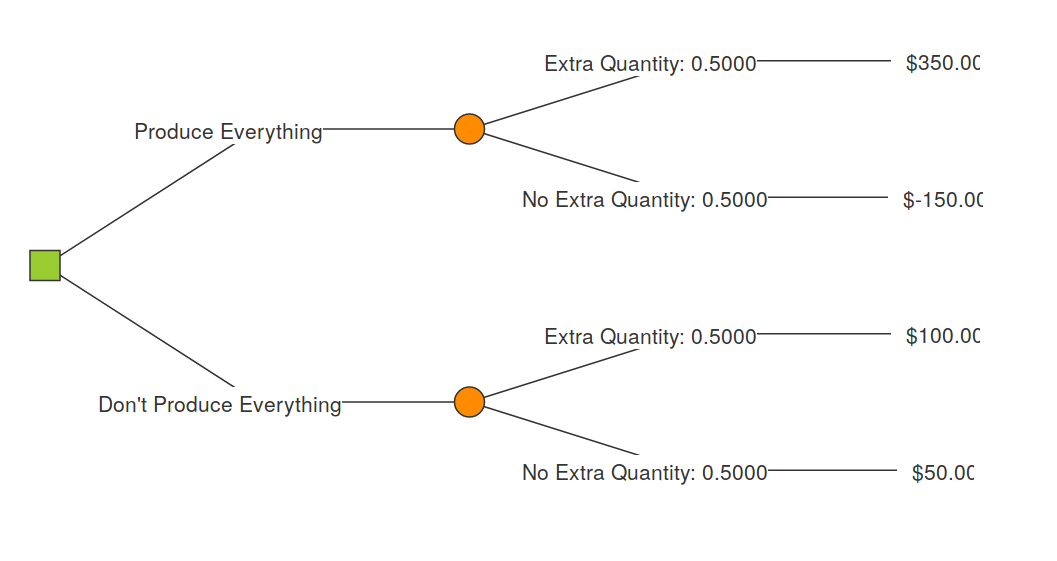
\includegraphics{Assignment1_files/figure-latex/EX1.png}

In the Decision Tree initially \emph{MC Manufacturing} need to choose
either to produce the whole batch of \(200,000\) pieces toghether or to
do it in two different moments, each time \emph{MC Manufacturing} starts
the batch production procedure, as mentioned in the introduction,
\emph{MC Manufacturing} pays \(\$250,000\), \emph{MC Manufacturing} does
not know if \emph{DISCO Electronics} will buy the second batch, but
\emph{MC Manufacturing} knows its the probability. Also we assume that
\emph{MC Manufacturing} does not have an option to produce \(0\)
quantity since in introduction we have that the contract has already
been made. In the decision tree above we can see the initial choice to
produce everything or not to produce everything and wait for the
decision of \emph{DISCO Electronics}, in both branches we have a chance
node to indicate possibity that \emph{DISCO Electronics} will ask for
another \(100,000\) PC boards or not. We choose to scale the values by
\(1,000\) to have smaller number during the calculations, so a profit of
\(\$350\) indicates a profit of \(\$350,000\). One thing we note
immediately is that the alternative to produce everything toghether
avoids the setup cost of \(\$250,000\) twice but at the same moment it
is the most risky one, since we have \(50\%\) probability to have a loss
of \(\$150,000\).

\subsection{Expected value}\label{expected-value}

\begin{itemize}
\tightlist
\item
  Determine the preferred course of action for MC assuming it uses
  expected profit as its decision criterion.
\end{itemize}

\subsubsection{Solution}\label{solution-1}

\begin{Shaded}
\begin{Highlighting}[]
\KeywordTok{plot}\NormalTok{(result, }\DataTypeTok{final =} \OtherTok{TRUE}\NormalTok{)}
\end{Highlighting}
\end{Shaded}

\hypertarget{htmlwidget-38dae67af6b8ac6c79d4}{}

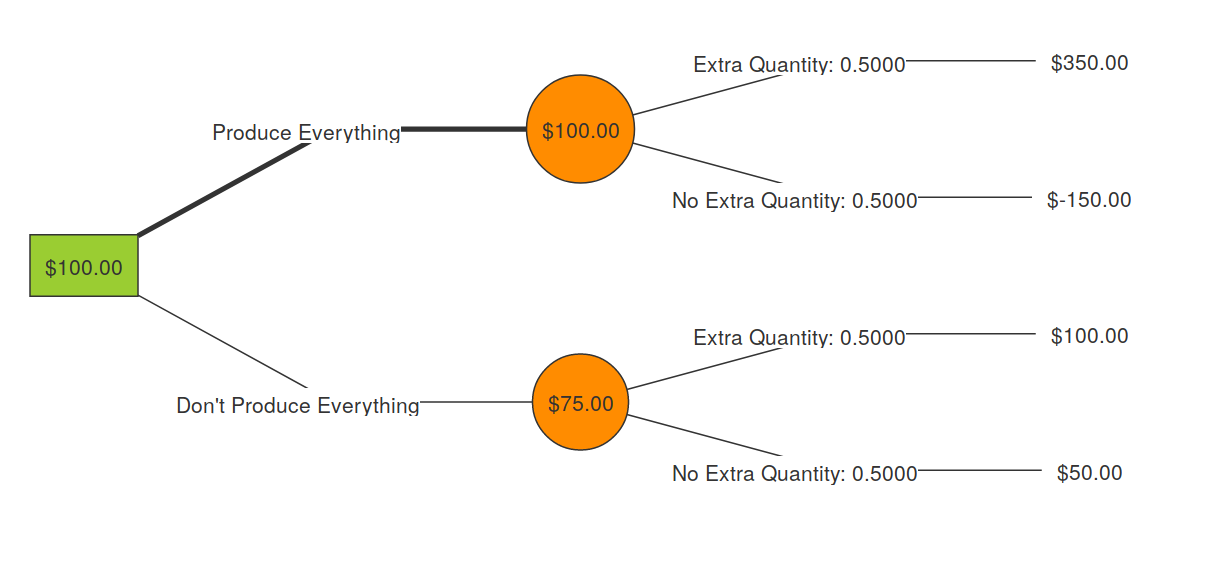
\includegraphics{Assignment1_files/figure-latex/EX2.png}

From the decision tree we can see that the preferred course of action is
to produce the two batches toghether since it has an expected value of
\(\$100,000\) against \(\$75,000\) of the other branch in which \emph{MC
Manufacturing} produces the two batch separately.

\subsection{Utility Function and Certainty
Equivalent}\label{utility-function-and-certainty-equivalent}

Assume that all the information still holds, except assume now that MC
has an exponential utility function with a risk tolerance of
\(\$100,000\).

We start by defining the functions that will be needed for the solution.

\begin{Shaded}
\begin{Highlighting}[]
\NormalTok{utilityFunctionExp <-}\StringTok{ }\ControlFlowTok{function}\NormalTok{(X, R) \{}
  \KeywordTok{return}\NormalTok{(}\DecValTok{1}\OperatorTok{-}\StringTok{ }\KeywordTok{exp}\NormalTok{(}\OperatorTok{-}\NormalTok{X}\OperatorTok{/}\NormalTok{R))}
\NormalTok{\}}

\NormalTok{CertEquivalent <-}\StringTok{ }\ControlFlowTok{function}\NormalTok{(EU, R)\{}
  \KeywordTok{return}\NormalTok{(}\OperatorTok{-}\NormalTok{R}\OperatorTok{*}\KeywordTok{ln}\NormalTok{(}\DecValTok{1}\OperatorTok{-}\NormalTok{EU))}
\NormalTok{\}}

\NormalTok{CalcExpectedUtilityFunction <-}\StringTok{ }\ControlFlowTok{function}\NormalTok{(profit, R)\{}
  \CommentTok{#------Branch 1----------#}
\NormalTok{  UF1 <-}\StringTok{ }\KeywordTok{utilityFunctionExp}\NormalTok{(profit}\OperatorTok{$}\NormalTok{profitBranch1, R)}
\NormalTok{  EU1 <-}\StringTok{ }\NormalTok{UF1[}\DecValTok{1}\NormalTok{]}\OperatorTok{*}\FloatTok{0.5} \OperatorTok{+}\StringTok{ }\NormalTok{UF1[}\DecValTok{2}\NormalTok{]}\OperatorTok{*}\FloatTok{0.5} \CommentTok{#Expected Utility Branch 1}

  \CommentTok{#------Branch 2----------#}
\NormalTok{  UF2 <-}\StringTok{ }\KeywordTok{utilityFunctionExp}\NormalTok{(profit}\OperatorTok{$}\NormalTok{profitBranch2, R)}
\NormalTok{  EU2 <-}\StringTok{ }\NormalTok{UF2[}\DecValTok{1}\NormalTok{]}\OperatorTok{*}\FloatTok{0.5} \OperatorTok{+}\StringTok{ }\NormalTok{UF2[}\DecValTok{2}\NormalTok{]}\OperatorTok{*}\FloatTok{0.5} \CommentTok{#Expected Utility Branch 2}
  
  \CommentTok{#----Return Final Result----#}
  \KeywordTok{return}\NormalTok{(}\KeywordTok{c}\NormalTok{(EU1, EU2))}
\NormalTok{\}}

\NormalTok{CalcBranchCE <-}\StringTok{ }\ControlFlowTok{function}\NormalTok{(profit, R)\{}
\NormalTok{CE_vett <-}\StringTok{ }\KeywordTok{CertEquivalent}\NormalTok{(}\KeywordTok{CalcExpectedUtilityFunction}\NormalTok{(profit, R), R)}
\KeywordTok{return}\NormalTok{(CE_vett)}
\NormalTok{\}}

\CommentTok{#Create a DataFrame with Profits per Branch}

\NormalTok{index <-}\StringTok{ }\DecValTok{1}\OperatorTok{:}\DecValTok{2}
\NormalTok{profitBranch1 <-}\StringTok{ }\KeywordTok{c}\NormalTok{(}\DecValTok{350}\NormalTok{,}\OperatorTok{-}\DecValTok{150}\NormalTok{)}
\NormalTok{profitBranch2 <-}\StringTok{ }\KeywordTok{c}\NormalTok{(}\DecValTok{100}\NormalTok{,}\DecValTok{50}\NormalTok{)}
\NormalTok{profit <-}\StringTok{ }\KeywordTok{data.frame}\NormalTok{(}\StringTok{"X"}\NormalTok{=index,}\StringTok{"profitBranch1"}\NormalTok{=profitBranch1,}\StringTok{"profitBranch2"}\NormalTok{=profitBranch2)}
\NormalTok{R=}\DecValTok{100} \CommentTok{#Remeber we scaled everything by 1000, so the R goes from 100,000 to 100}
\end{Highlighting}
\end{Shaded}

\begin{itemize}
\tightlist
\item
  Determine MC's preferred course of action.
\end{itemize}

\subsubsection{Solution}\label{solution-2}

\begin{Shaded}
\begin{Highlighting}[]
\NormalTok{CE <-}\StringTok{ }\KeywordTok{CalcBranchCE}\NormalTok{(profit,R)}

\NormalTok{CE_Branch1 <-}\StringTok{ }\NormalTok{CE[}\DecValTok{1}\NormalTok{]}\OperatorTok{*}\DecValTok{1000}
\NormalTok{CE_Branch2 <-}\StringTok{ }\NormalTok{CE[}\DecValTok{2}\NormalTok{]}\OperatorTok{*}\DecValTok{1000}
\KeywordTok{cat}\NormalTok{(}\KeywordTok{paste0}\NormalTok{(}\StringTok{'Certainty Equivalent of Branch of producing eveything together: '}\NormalTok{,CE_Branch1),}
    \KeywordTok{paste0}\NormalTok{(}\StringTok{'Certainty Equivalent of Branch of producing separately: '}\NormalTok{,CE_Branch2),}
    \StringTok{'NOTE: The values are re-scaled to the right scale.'}\NormalTok{,}
    \StringTok{'********************************************************'}\NormalTok{,}\DataTypeTok{sep=}\StringTok{'}\CharTok{\textbackslash{}n}\StringTok{'}\NormalTok{)}
\end{Highlighting}
\end{Shaded}

\begin{verbatim}
Certainty Equivalent of Branch of producing eveything together: -81356.8167929173
Certainty Equivalent of Branch of producing separately: 71907.0196379839
NOTE: The values are re-scaled to the right scale.
********************************************************
\end{verbatim}

We can see that the preferred course is now the Branch in which we wait
before producing the other batch. We have that the Certainty Equivalent
in this case is \(\$71907\), which is smaller than the expected value
thus in this case \emph{MC Manufacturing} is risk averse.

Since the difference between the Certainty Equivalent of the two
branches is so high, we can say that for a large neighborhood (interval
of a value) of \(R = 100,000\) we will have that the preferred branch
will be the one in which we wait to produce the other batch. Actually
from the plot below we have that the preferred choice is to wait before
producing everything until a very big value of R (between \(1,100,000\)
and \(1,300,000\)). This change of preference is there since for large R
we become more risk seeking.

\begin{Shaded}
\begin{Highlighting}[]
\NormalTok{R =}\StringTok{ }\KeywordTok{seq}\NormalTok{(}\DecValTok{2}\NormalTok{, }\DecValTok{1300}\NormalTok{, }\DecValTok{1}\NormalTok{)}
\NormalTok{res1 =}\StringTok{ }\KeywordTok{c}\NormalTok{()}
\NormalTok{res2 =}\StringTok{ }\KeywordTok{c}\NormalTok{()}
\ControlFlowTok{for}\NormalTok{ (i }\ControlFlowTok{in} \DecValTok{1}\OperatorTok{:}\KeywordTok{length}\NormalTok{(R)) \{}
\NormalTok{vRes =}\StringTok{ }\KeywordTok{CalcBranchCE}\NormalTok{(profit, R[i])}
\NormalTok{res1[i] =}\StringTok{ }\NormalTok{vRes[}\DecValTok{1}\NormalTok{]}
\NormalTok{res2[i] =}\StringTok{ }\NormalTok{vRes[}\DecValTok{2}\NormalTok{]}
\NormalTok{\}}
\KeywordTok{plot}\NormalTok{(R, res1, }\DataTypeTok{type=}\StringTok{"l"}\NormalTok{, }\DataTypeTok{col=}\StringTok{"blue"}\NormalTok{, }\DataTypeTok{ylab=}\StringTok{"CE(scaled by 1000)"}\NormalTok{, }\DataTypeTok{xlab =} \StringTok{"R(scaled by 1000)"}\NormalTok{,}
     \DataTypeTok{xlim=}\KeywordTok{c}\NormalTok{(}\OperatorTok{-}\DecValTok{1}\NormalTok{, }\KeywordTok{max}\NormalTok{(R)}\OperatorTok{+}\DecValTok{1}\NormalTok{), }\DataTypeTok{ylim=}\KeywordTok{c}\NormalTok{(}\KeywordTok{min}\NormalTok{(res1), }\KeywordTok{max}\NormalTok{(res2)))}
\KeywordTok{points}\NormalTok{ (R, res2, }\DataTypeTok{type=}\StringTok{"l"}\NormalTok{, }\DataTypeTok{col=}\StringTok{"red"}\NormalTok{)}
\KeywordTok{legend}\NormalTok{(}\DecValTok{500}\NormalTok{,}\OperatorTok{-}\DecValTok{50}\NormalTok{,}\DataTypeTok{legend=}\KeywordTok{c}\NormalTok{(}\StringTok{'Produce Separately'}\NormalTok{,}\StringTok{'Produce Together'}\NormalTok{),}\DataTypeTok{col=}\KeywordTok{c}\NormalTok{(}\StringTok{"red"}\NormalTok{, }\StringTok{"blue"}\NormalTok{), }\DataTypeTok{lty=}\DecValTok{1}\NormalTok{)}
\end{Highlighting}
\end{Shaded}

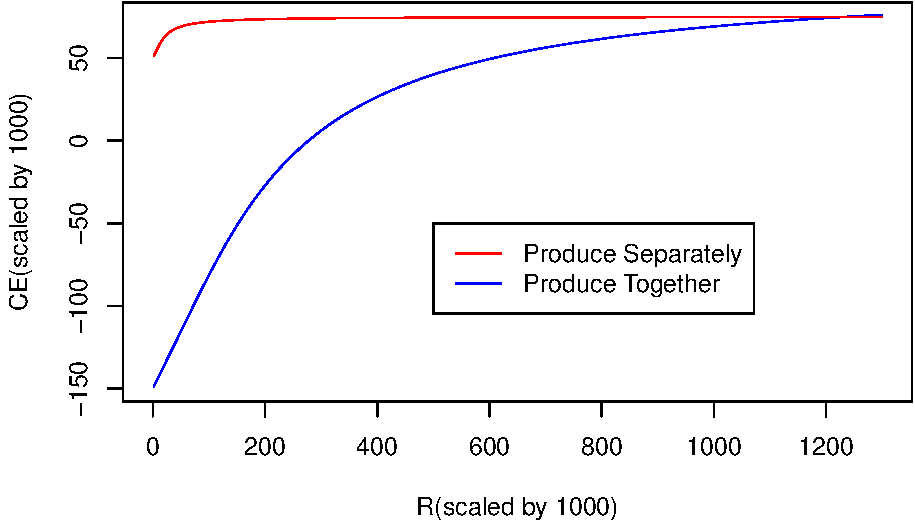
\includegraphics{Assignment1_files/figure-latex/interval of R-1.pdf}

\subsection{Modification of the
process}\label{modification-of-the-process}

For the decision in the preceding point, MC Manufacturing has created a
new option: it can conduct some research and development in an attempt
to lower the fixed setup cost associated with manufacturing a batch of
the PC boards. This research and development would not be completed in
time to influence the setup cost for the initial batch that DISCO has
ordered, but would be completed before the second batch would have to be
manufactured. The research and development will cost \(\$25,000\), and
there is a 0.4 probability that it will be successful. If it is
successful, then the fixed setup cost per batch will be reduced by
\(\$200,000\) to \(\$50,000\). If the research and development is not
successful, then there will be no reduction in the setup cost. There
will be no other benefits from the research and development besides the
potential reduction in setup cost for the DISCO reorder.

\begin{itemize}
\tightlist
\item
  Using expected profit as the decision criterion, determine whether MC
  should undertake the research and development.
\end{itemize}

\subsubsection{Solution}\label{solution-3}

\begin{Shaded}
\begin{Highlighting}[]
\NormalTok{tree_RnD =}\StringTok{ }\KeywordTok{yaml.load_file}\NormalTok{(}\DataTypeTok{input =} \StringTok{"./Board_Production_RnD.yaml"}\NormalTok{)}
\NormalTok{result_RnD =}\StringTok{ }\KeywordTok{dtree}\NormalTok{(}\DataTypeTok{yl =}\NormalTok{ tree_RnD)}

\KeywordTok{plot}\NormalTok{(result_RnD, }\DataTypeTok{final =} \OtherTok{TRUE}\NormalTok{)}
\end{Highlighting}
\end{Shaded}

\hypertarget{htmlwidget-4fc2eb8b18d81d4d1453}{}

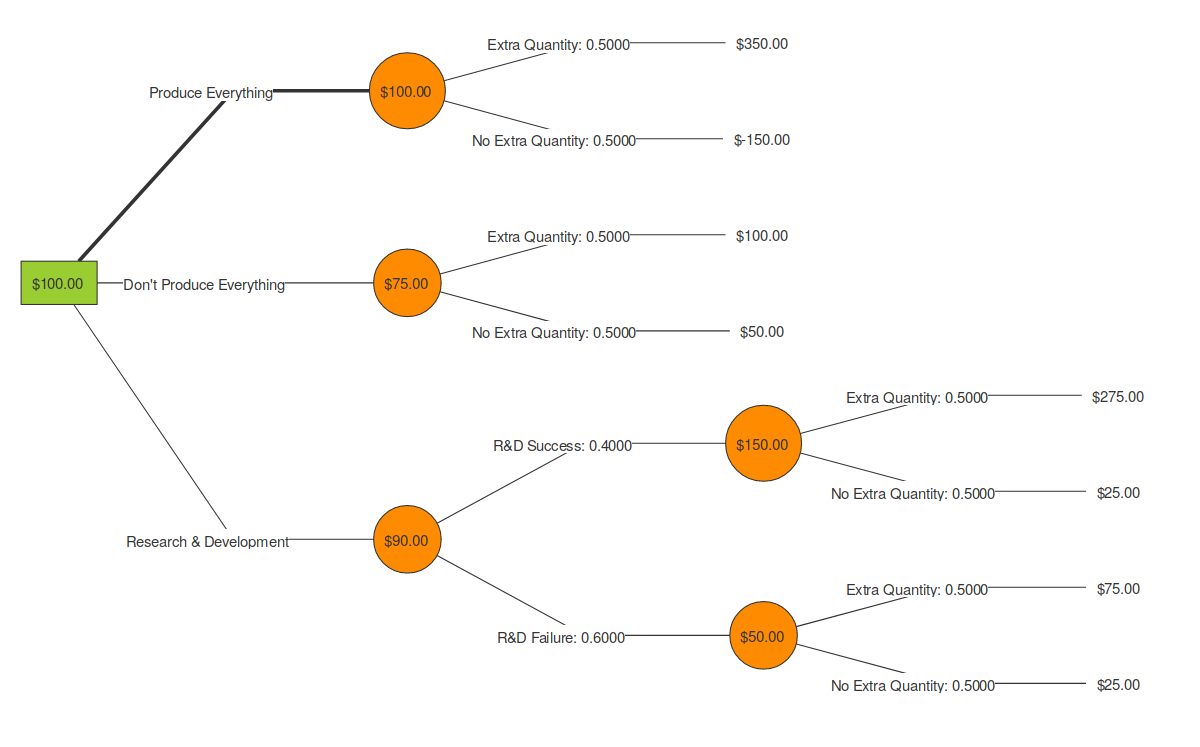
\includegraphics{Assignment1_files/figure-latex/EX4.png}

Since the R\&D will not be completed before the first batch, it would
not make any sense to research in case we choose to produce everything
toghether, since it would only extra cost without any benefit for the
company. So in case we undergo the R\&D(Research and Developement)
proccess we will consider only the case we were to produce the two batch
separately.

The R\&D branch has an Expected Value of \(\$90,000\) which is still
lower than the Branch in which we have a production of everything
toghether, so using the expected profit the preferred course is still
Branch of producing everything together, thus \emph{MC Manufacturing}
should not undertake the R\&D.

We decided to keep the two choices of Producing Separeptly (``Don't
Produce Everything'') and R\&D separated, one could have equivalently
created another decision node in the ``Don't Produce Everything'' branch
of either doing or not the R\&D.

\subsection{Value of Information}\label{value-of-information}

Using expected profit as the decision criteria, determine the value of
learning for certain whether the research and development will be
successful before a decision has to be made about whether to initially
manufacture \(100,000\) or \(200,000\) PC boards.

\subsubsection{Solution}\label{solution-4}

\begin{Shaded}
\begin{Highlighting}[]
\NormalTok{tree_PI =}\StringTok{ }\KeywordTok{yaml.load_file}\NormalTok{(}\DataTypeTok{input =} \StringTok{"./Board_Production_PI.yaml"}\NormalTok{)}
\NormalTok{result_PI =}\StringTok{ }\KeywordTok{dtree}\NormalTok{(}\DataTypeTok{yl =}\NormalTok{ tree_PI)}


\KeywordTok{plot}\NormalTok{(result_PI, }\DataTypeTok{final =} \OtherTok{TRUE}\NormalTok{)}
\end{Highlighting}
\end{Shaded}

\hypertarget{htmlwidget-f8756e2f3c4a367dd19b}{}

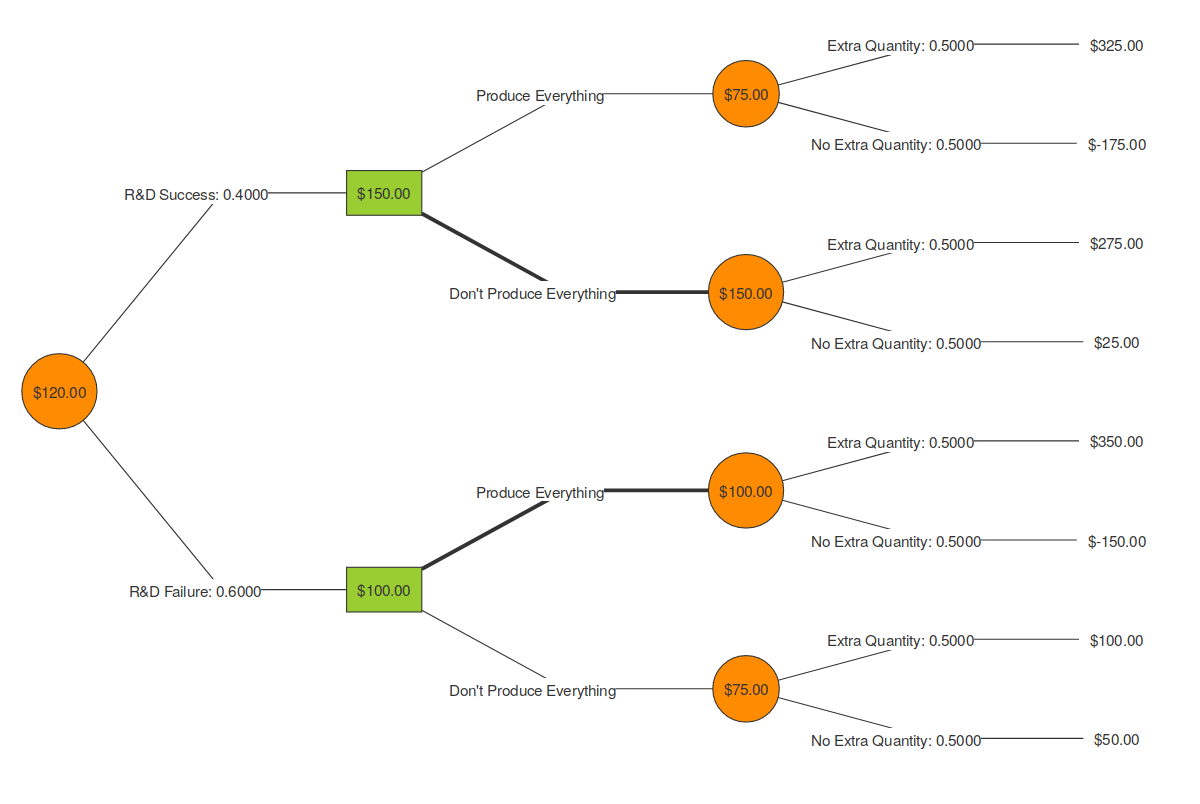
\includegraphics{Assignment1_files/figure-latex/EX5.png}

Since we are asked to determine the value of learning for certain the
information, we assume the information to be perfect, the Expected Value
using this perfetct information is \(\$120,000\) while the best expected
value without the information on the success of R\&D was \(\$100,000\),
since the value of information using the expected profit is the
difference between the two values, thus
\(\$120,000 - \$100,000 = \$20,000\) is the value of such information.

We also have that in case of the failure of R\&D, \emph{MC
Manufacturing} should decide to produce everything toghether, while in
the case of a successful R\&D \emph{MC Manufacturing} should produce the
two batches separately using as the measure expected value. In case of
the success of R\&D and after chosing to produce the two batch
separately we have that with a probability of \(50\%\) that the second
batch will not be needed, so the the research is useful only in one case
among a total of 8 possible cases, which is an information that \emph{MC
Manufacturing} should take in consideration.

In the model here we decided to show all the possible alternative, for
example in the case of failure of R\&D it would not make any sense to
Produce the boards separately since we already know from point 2 that
the other branch is more convenient in this case using as measure the
expected value. The choice was made so that, in case the company were to
decide to bargain/change any of the provided cost or revenue, we could
see it's repercussion on every branch. Another reason was the
completeness of the structure.

\pagebreak

\section{Appendix}\label{appendix}

Here we print the structure of the yaml file.

\subsection{Exercise 1}\label{exercise-1}

\begin{Shaded}
\begin{Highlighting}[]
\KeywordTok{summary}\NormalTok{(result, }\DataTypeTok{input =} \OtherTok{FALSE}\NormalTok{, }\DataTypeTok{output =} \OtherTok{TRUE}\NormalTok{)}
\end{Highlighting}
\end{Shaded}

\begin{verbatim}
Variable input values:
                                     
setup cost                      250.0
manufacture cost                200.0
unit_revenue                    500.0
prob_extra                        0.5
prob_not_extra                    0.5
cost_toghether_extra            650.0
cost_toghether_not_extra        650.0
cost_not_together_extra         900.0
cost_not_together_not_extra     450.0
revenue_extra                  1000.0
revenue_not_extra               500.0
payoff_toghether_extra          350.0
payoff_toghether_not_extra     -150.0
payoff_not_toghether_extra      100.0
payoff_not_toghether_not_extra   50.0

Initial decision tree:
                              Probability  Payoff Cost     Type
 Board Production Decision                                     
  ¦--Produce Everything                                decision
  ¦   ¦--Extra Quantity           50.00 %  350.00        chance
  ¦   °--No Extra Quantity        50.00 % -150.00        chance
  °--Don't Produce Everything                          decision
      ¦--Extra Quantity           50.00 %  100.00        chance
      °--No Extra Quantity        50.00 %   50.00        chance

Final decision tree:
                              Probability  Payoff Cost     Type
 Board Production Decision                 100.00              
  ¦--Produce Everything                    100.00      decision
  ¦   ¦--Extra Quantity           50.00 %  350.00        chance
  ¦   °--No Extra Quantity        50.00 % -150.00        chance
  °--Don't Produce Everything               75.00      decision
      ¦--Extra Quantity           50.00 %  100.00        chance
      °--No Extra Quantity        50.00 %   50.00        chance
\end{verbatim}

\subsection{Exercise 2}\label{exercise-2}

\begin{Shaded}
\begin{Highlighting}[]
\KeywordTok{summary}\NormalTok{(result_RnD, }\DataTypeTok{input =} \OtherTok{FALSE}\NormalTok{, }\DataTypeTok{output =} \OtherTok{TRUE}\NormalTok{)}
\end{Highlighting}
\end{Shaded}

\begin{verbatim}
Variable input values:
                                     
setup_cost                      250.0
manufacture_cost                200.0
research_cost                    25.0
setup_RnD_cost                   50.0
unit_revenue                    500.0
prob_extra                        0.5
prob_not_extra                    0.5
prob_RnD_success                  0.4
prob_RnD_fail                     0.6
cost_toghether_extra            650.0
cost_toghether_not_extra        650.0
cost_not_together_extra         900.0
cost_not_together_not_extra     450.0
revenue_extra                  1000.0
revenue_not_extra               500.0
payoff_toghether_extra          350.0
payoff_toghether_not_extra     -150.0
payoff_not_toghether_extra      100.0
payoff_not_toghether_not_extra   50.0
cost_RnD_success_extra          725.0
cost_RnD_success_not_extra      475.0
cost_RnD_fail_extra             925.0
cost_RnD_fail_not_extra         475.0
payoff_RnD_success_extra        275.0
payoff_RnD_success_not_extra     25.0
payoff_RnD_fail_extra            75.0
payoff_RnD_fail_not_extra        25.0

Initial decision tree:
                               Probability  Payoff Cost     Type
 Board Production Decision RnD                                  
  ¦--Produce Everything                                 decision
  ¦   ¦--Extra Quantity            50.00 %  350.00        chance
  ¦   °--No Extra Quantity         50.00 % -150.00        chance
  ¦--Don't Produce Everything                           decision
  ¦   ¦--Extra Quantity            50.00 %  100.00        chance
  ¦   °--No Extra Quantity         50.00 %   50.00        chance
  °--Research & Development                             decision
      ¦--R&D Success               40.00 %                chance
      ¦   ¦--Extra Quantity        50.00 %  275.00        chance
      ¦   °--No Extra Quantity     50.00 %   25.00        chance
      °--R&D Failure               60.00 %                chance
          ¦--Extra Quantity        50.00 %   75.00        chance
          °--No Extra Quantity     50.00 %   25.00        chance

Final decision tree:
                               Probability  Payoff Cost     Type
 Board Production Decision RnD              100.00              
  ¦--Produce Everything                     100.00      decision
  ¦   ¦--Extra Quantity            50.00 %  350.00        chance
  ¦   °--No Extra Quantity         50.00 % -150.00        chance
  ¦--Don't Produce Everything                75.00      decision
  ¦   ¦--Extra Quantity            50.00 %  100.00        chance
  ¦   °--No Extra Quantity         50.00 %   50.00        chance
  °--Research & Development                  90.00      decision
      ¦--R&D Success               40.00 %  150.00        chance
      ¦   ¦--Extra Quantity        50.00 %  275.00        chance
      ¦   °--No Extra Quantity     50.00 %   25.00        chance
      °--R&D Failure               60.00 %   50.00        chance
          ¦--Extra Quantity        50.00 %   75.00        chance
          °--No Extra Quantity     50.00 %   25.00        chance
\end{verbatim}

\subsection{Exercise 3}\label{exercise-3}

\begin{Shaded}
\begin{Highlighting}[]
\KeywordTok{summary}\NormalTok{(result_PI, }\DataTypeTok{input =} \OtherTok{FALSE}\NormalTok{, }\DataTypeTok{output =} \OtherTok{TRUE}\NormalTok{)}
\end{Highlighting}
\end{Shaded}

\begin{verbatim}
Variable input values:
                                             
setup_cost                              250.0
manifacture_cost                        200.0
setup_RnD_cost                           50.0
research_cost                            25.0
unit_revenue                            500.0
prob_extra                                0.5
prob_not_extra                            0.5
prob_RnD_success                          0.4
prob_RnD_fail                             0.6
revenue_extra                          1000.0
revenue_not_extra                       500.0
cost_success_toghether_extra            675.0
cost_success_toghether_not_extra        675.0
cost_success_not_toghether_extra        725.0
cost_success_not_toghether_not_extra    475.0
payoff_success_toghether_extra          325.0
payoff_success_toghether_not_extra     -175.0
payoff_success_not_toghether_extra      275.0
payoff_success_not_toghether_not_extra   25.0
cost_fail_toghether_extra               650.0
cost_fail_toghether_not_extra           650.0
cost_fail_not_toghether_extra           900.0
cost_fail_not_toghether_not_extra       450.0
payoff_fail_toghether_extra             350.0
payoff_fail_toghether_not_extra        -150.0
payoff_fail_not_toghether_extra         100.0
payoff_fail_not_toghether_not_extra      50.0

Initial decision tree:
                                  Probability  Payoff Cost     Type
 Board Production Decision RnD                                     
  ¦--R&D Success                      40.00 %                chance
  ¦   ¦--Produce Everything                                decision
  ¦   ¦   ¦--Extra Quantity           50.00 %  325.00        chance
  ¦   ¦   °--No Extra Quantity        50.00 % -175.00        chance
  ¦   °--Don't Produce Everything                          decision
  ¦       ¦--Extra Quantity           50.00 %  275.00        chance
  ¦       °--No Extra Quantity        50.00 %   25.00        chance
  °--R&D Failure                      60.00 %                chance
      ¦--Produce Everything                                decision
      ¦   ¦--Extra Quantity           50.00 %  350.00        chance
      ¦   °--No Extra Quantity        50.00 % -150.00        chance
      °--Don't Produce Everything                          decision
          ¦--Extra Quantity           50.00 %  100.00        chance
          °--No Extra Quantity        50.00 %   50.00        chance

Final decision tree:
                                  Probability  Payoff Cost     Type
 Board Production Decision RnD                 120.00              
  ¦--R&D Success                      40.00 %  150.00        chance
  ¦   ¦--Produce Everything                     75.00      decision
  ¦   ¦   ¦--Extra Quantity           50.00 %  325.00        chance
  ¦   ¦   °--No Extra Quantity        50.00 % -175.00        chance
  ¦   °--Don't Produce Everything              150.00      decision
  ¦       ¦--Extra Quantity           50.00 %  275.00        chance
  ¦       °--No Extra Quantity        50.00 %   25.00        chance
  °--R&D Failure                      60.00 %  100.00        chance
      ¦--Produce Everything                    100.00      decision
      ¦   ¦--Extra Quantity           50.00 %  350.00        chance
      ¦   °--No Extra Quantity        50.00 % -150.00        chance
      °--Don't Produce Everything               75.00      decision
          ¦--Extra Quantity           50.00 %  100.00        chance
          °--No Extra Quantity        50.00 %   50.00        chance
\end{verbatim}


\end{document}
